% Rapport technique – Projet intégré « Système de contrôle-commande Dual-UI »
% Compilation : xelatex rapport.tex (deux fois)   – ou `make livrables` à la racine du dépôt
\documentclass[11pt,a4paper]{article}

\usepackage{fontspec}
\setmainfont{Noto Serif}
\setsansfont{Noto Sans}
\setmonofont{Noto Sans Mono}[Scale=0.85]
\usepackage[french]{babel}
\usepackage[a4paper,margin=2cm]{geometry}
\usepackage{graphicx,xcolor,booktabs,tabularx,array,enumitem,float,caption,subcaption}
\usepackage{listings,tikz,fancyhdr,titlesec,microtype}
\usepackage[hidelinks]{hyperref}
\usetikzlibrary{positioning,arrows.meta,shapes.geometric,fit,calc}

\graphicspath{{figures/captures/}{figures/wireframes/}}
\definecolor{accent}{HTML}{1D6FB8}
\definecolor{ok}{HTML}{1E8A4C}
\definecolor{partiel}{HTML}{B7791F}
\definecolor{non}{HTML}{C0392B}
\definecolor{codebg}{HTML}{F6F8FA}
\newcommand{\ok}{\textcolor{ok}{\textbf{Oui}}}
\newcommand{\partiel}{\textcolor{partiel}{\textbf{Partiel}}}
\newcommand{\non}{\textcolor{non}{\textbf{Non}}}
\newcommand{\hors}{\textcolor{gray}{\textbf{Hors périmètre}}}

\titleformat{\section}{\sffamily\Large\bfseries\color{accent}}{\thesection.}{0.5em}{}
\titleformat{\subsection}{\sffamily\large\bfseries}{\thesubsection}{0.5em}{}
\setlist{nosep,leftmargin=1.4em}
\setlength{\parskip}{0.45em}
\setlength{\parindent}{0pt}
\captionsetup{font=small,labelfont=bf}

\pagestyle{fancy}
\fancyhf{}
\fancyhead[L]{\small\sffamily Station de sécurité Raspberry Pi -- Rapport technique}
\fancyhead[R]{\small\sffamily M. Robison -- 5A ESE}
\fancyfoot[C]{\small\thepage}

\lstset{
  language=Python, basicstyle=\ttfamily\footnotesize, backgroundcolor=\color{codebg},
  frame=single, rulecolor=\color{black!15}, numbers=left, numberstyle=\tiny\color{gray},
  keywordstyle=\color{accent}\bfseries, commentstyle=\color{gray}\itshape,
  stringstyle=\color{ok!80!black}, showstringspaces=false, breaklines=true,
  xleftmargin=1.5em, framexleftmargin=1.5em, aboveskip=0.6em, belowskip=0.4em,
}
\newcommand{\src}[1]{../../security_station/#1}

\begin{document}

% ======================================================================= page de garde
\begin{titlepage}
  \centering
  \vspace*{1cm}
  {\sffamily\large INSA Hauts-de-France -- Électronique et Systèmes Embarqués\par}
  {\sffamily 5A ESE -- Prototypage des systèmes embarqués\par}
  \vspace{2.5cm}
  {\sffamily\Huge\bfseries\color{accent} Station de sécurité\\[0.2em] Raspberry Pi\par}
  \vspace{0.6cm}
  {\sffamily\Large Projet intégré : système de contrôle-commande Dual-UI\par}
  \vspace{0.4cm}
  {\large Rapport technique -- phase de simulation logicielle (SIL)\par}
  \vspace{1.2cm}
  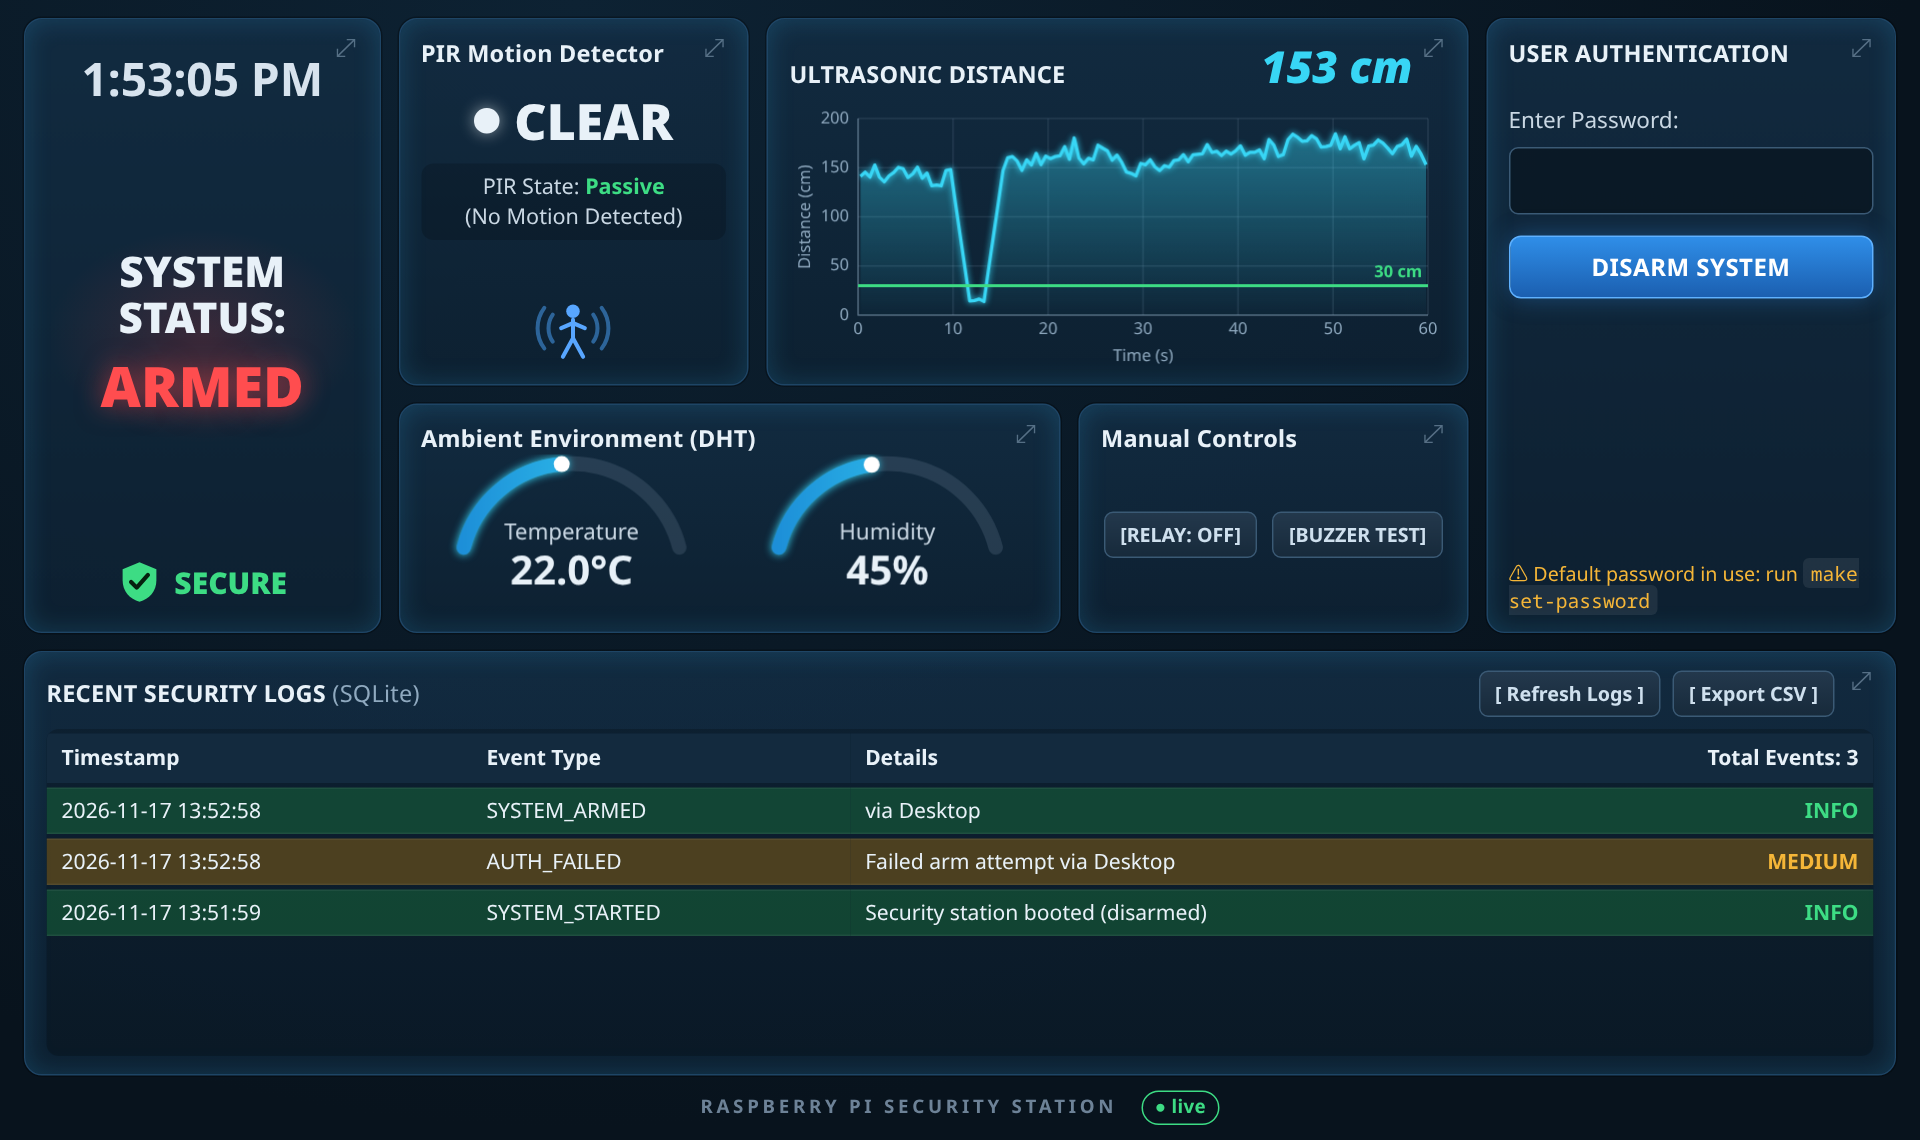
\includegraphics[width=0.85\linewidth]{web_2_normal.png}
  \vfill
  {\large\textbf{Marc Robison}\par}
  \vspace{0.3cm}
  Enseignant : M. Alain Allouis\par
  17 novembre 2026
\end{titlepage}

% ======================================================================= introduction
\section*{Introduction}
Le projet est une \textbf{station de sécurité} pour la maison. Elle surveille une pièce avec trois capteurs
et peut déclencher deux actionneurs :

\begin{itemize}
  \item \textbf{Capteur ultrason} (HC-SR04) : mesure la distance devant lui. En dessous de 30~cm, c'est une intrusion.
  \item \textbf{Détecteur de mouvement PIR} (HC-SR501) : détecte une présence dans la zone A ou B.
  \item \textbf{Capteur d'ambiance} (DHT22) : température et humidité.
  \item \textbf{Actionneurs} : un relais (par ex. une serrure ou une lampe) et un buzzer d'alarme.
\end{itemize}

On peut piloter la station de deux façons, en même temps :
\begin{itemize}
  \item sur l'écran de la Raspberry Pi, avec une \textbf{interface Qt} (PySide6) ;
  \item depuis un PC ou un téléphone sur le même Wi-Fi, avec une \textbf{interface web}.
\end{itemize}
Les deux interfaces affichent toujours la même chose. Une action faite sur l'une apparaît tout de suite sur l'autre.

\textbf{Périmètre.} Ce rapport couvre la phase de \textbf{simulation} (phase II). Les valeurs des capteurs
sont générées par logiciel. La phase matérielle (câblage, pilotes réels, vidéo de démonstration physique)
n'a pas été réalisée. Les textes de l'application sont en anglais.

% ======================================================================= partie 1
\newpage
\section{Architecture et UX}

\subsection{Parcours utilisateur}
\begin{figure}[H]
\centering
\begin{tikzpicture}[
  font=\sffamily\scriptsize,
  b/.style={draw, rounded corners=2pt, align=center, minimum height=8mm, inner sep=3pt},
  s/.style={b, fill=accent!10},
  a/.style={b, fill=non!10},
  arr/.style={-{Stealth[length=2mm]}, thick}]
  \node[b, minimum height=14mm, minimum width=22mm] (dash) at (0,0) {\textbf{Tableau de bord}\\7 tuiles};
  \node[s, minimum width=24mm] (pi)  at (-3.6, 0.6) {Écran Pi (Qt, plein écran)};
  \node[s, minimum width=24mm] (nav) at (-3.6,-0.6) {Navigateur (PC / téléphone)};
  \node[b, anchor=west] (tile) at (2.0, 1.1) {Clic sur une tuile};
  \node[b, right=5mm of tile] (big) {Vue agrandie};
  \node[b, right=5mm of big] (back) {« Back » ou Échap};
  \node[b, anchor=west] (pw) at (2.0, 0) {Mot de passe + ARM / DISARM};
  \node[b, right=5mm of pw] (fb) {Message vert ou rouge};
  \node[a, anchor=west] (al) at (2.0,-1.1) {Alarme (système)};
  \node[a, right=5mm of al] (st) {ALERT + buzzer + ligne au journal};
  \draw[arr] (pi.east) -- (dash.west |- pi.east);
  \draw[arr] (nav.east) -- (dash.west |- nav.east);
  \draw[arr] (dash.east) ++(0,0.3) -- ++(0.4,0) |- (tile.west);
  \draw[arr] (dash.east) -- (pw.west);
  \draw[arr] (dash.east) ++(0,-0.3) -- ++(0.4,0) |- (al.west);
  \draw[arr] (tile) -- (big); \draw[arr] (big) -- (back);
  \draw[arr] (pw) -- (fb); \draw[arr] (al) -- (st);
\end{tikzpicture}
\caption{Les trois parcours principaux, identiques sur Qt et sur le web.}
\end{figure}

\subsection{Maquettes basse fidélité}
\begin{figure}[H]
\centering
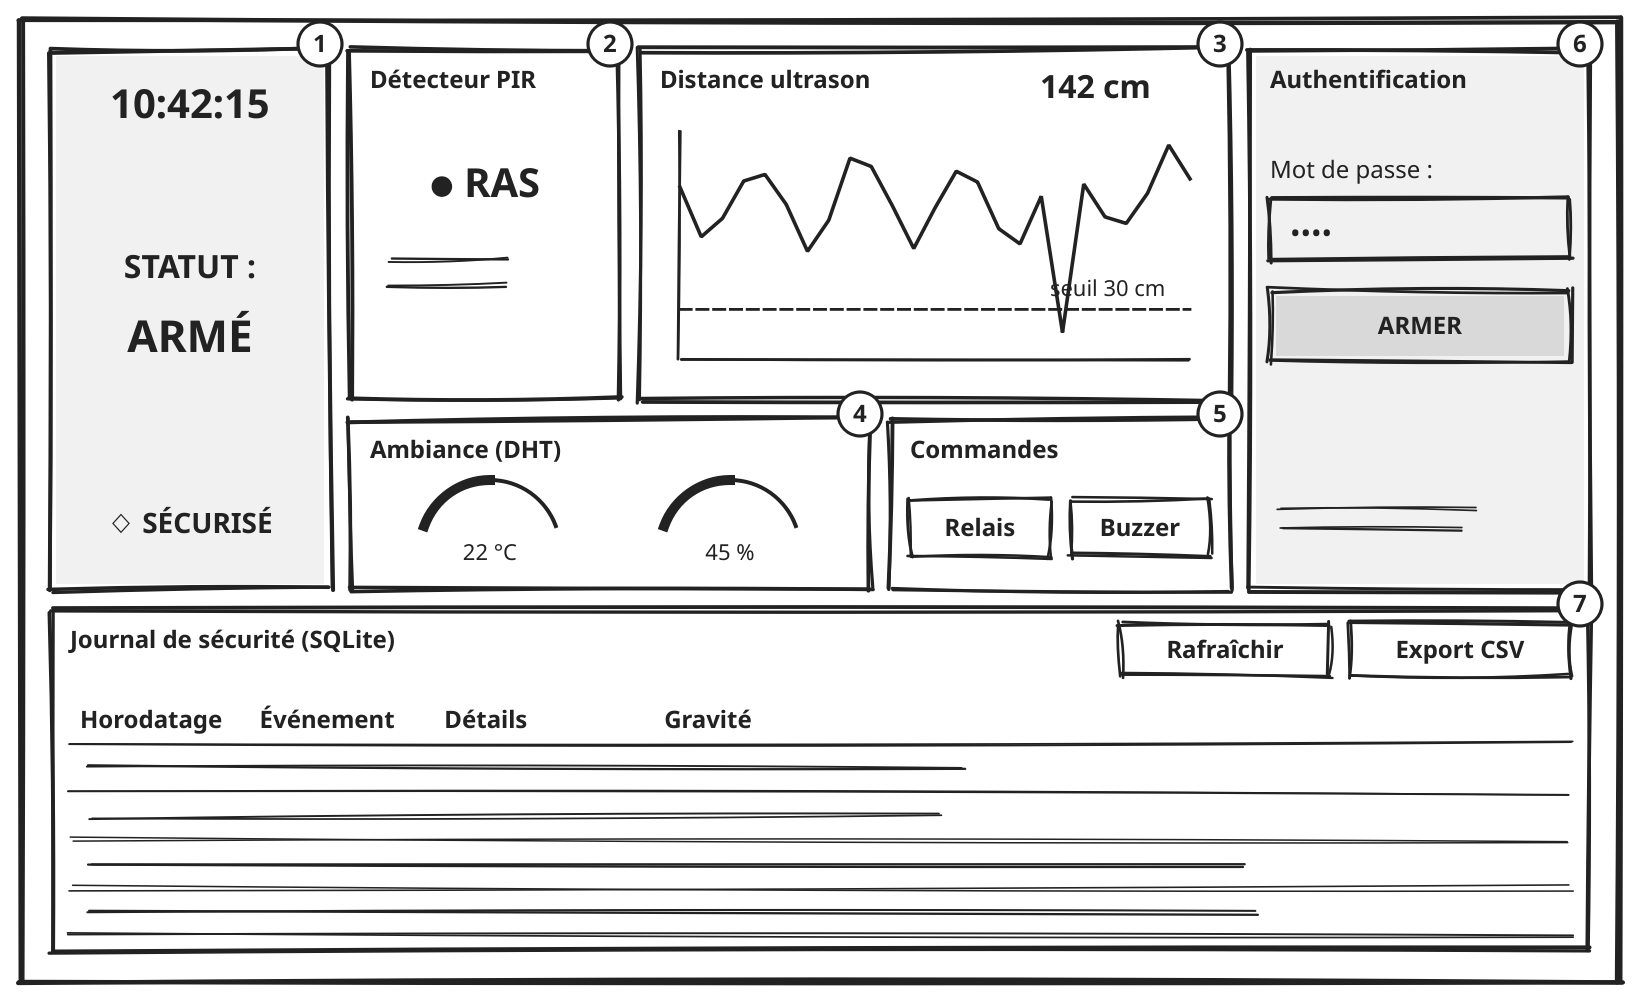
\includegraphics[width=0.74\linewidth]{wf_principal.png}
\caption{Écran principal (Qt et web sur PC). \textbf{1}~horloge et statut,
\textbf{2}~PIR, \textbf{3}~distance + seuil, \textbf{4}~température/humidité,
\textbf{5}~commandes, \textbf{6}~mot de passe, \textbf{7}~journal. Chaque tuile s'agrandit au clic.}
\end{figure}

\begin{figure}[H]
\centering
\begin{subfigure}[b]{0.52\linewidth}\centering
  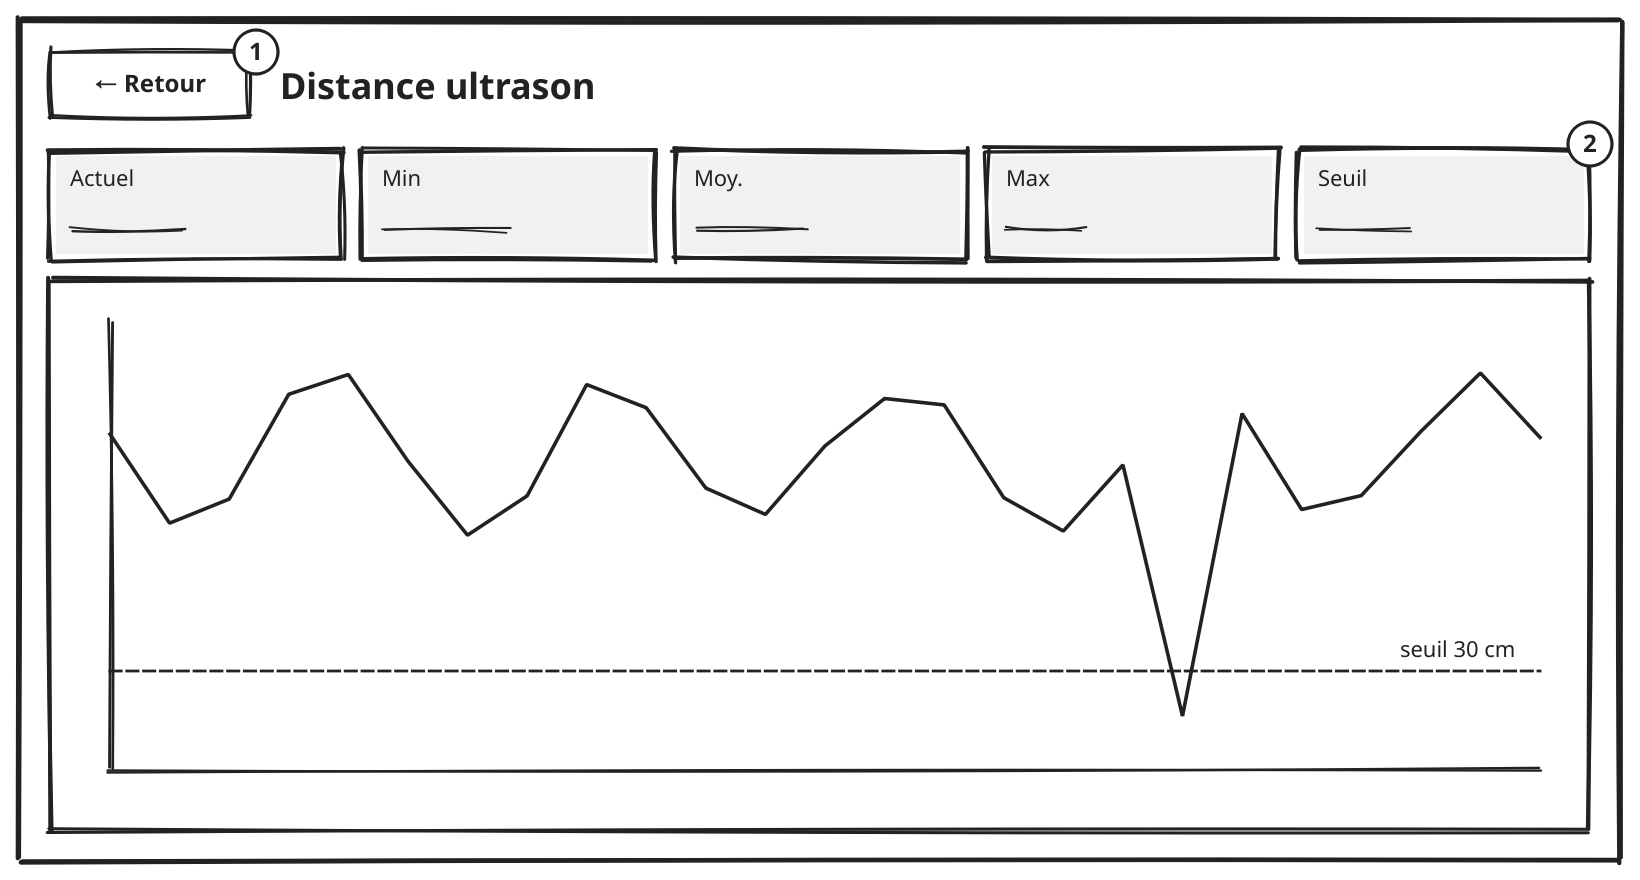
\includegraphics[width=\linewidth]{wf_agrandie.png}
  \caption{Tuile agrandie : bouton retour, chiffres clés, grand graphique.}
\end{subfigure}\hfill
\begin{subfigure}[b]{0.17\linewidth}\centering
  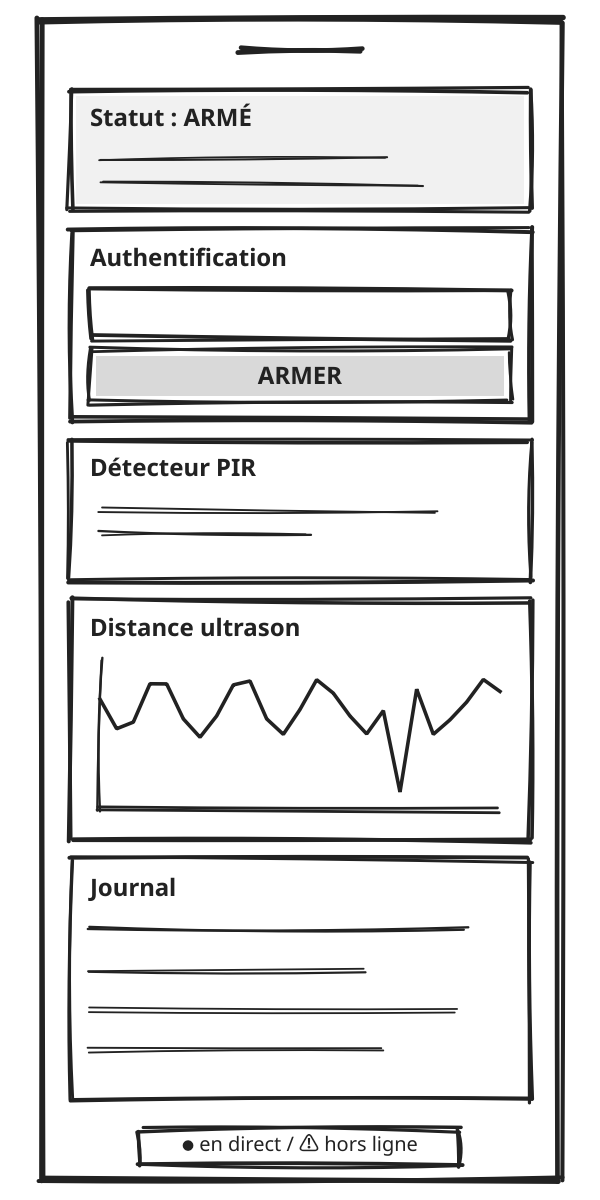
\includegraphics[width=\linewidth]{wf_mobile.png}
  \caption{Web sur téléphone : une seule colonne.}
\end{subfigure}
\caption{Vue agrandie et version mobile.}
\end{figure}

\textbf{Schéma de câblage :} hors périmètre, car la phase matérielle n'a pas été réalisée.

\subsection{Micro-interactions}
Trois moments clés, décrits avec le modèle de Dan Saffer :

\begin{table}[H]
\centering\small
\renewcommand{\arraystretch}{1.25}
\begin{tabularx}{\linewidth}{>{\bfseries\raggedright}p{2.1cm} >{\raggedright\arraybackslash}X >{\raggedright\arraybackslash}X >{\raggedright\arraybackslash}X}
\toprule
 & \textbf{1. Alarme d'intrusion} & \textbf{2. Armer / désarmer} & \textbf{3. Commander un actionneur} \\
\midrule
Déclencheur &
  \emph{Système} : un objet passe sous 30~cm, ou le PIR détecte un mouvement, alors que la station est armée. &
  \emph{Manuel} : l'utilisateur tape le mot de passe et appuie sur « ARM / DISARM SYSTEM ». &
  \emph{Manuel} : clic sur « RELAY » ou « BUZZER TEST », puis mot de passe dans une petite fenêtre. \\
Règles &
  On compare la valeur au seuil. On enregistre l'événement avec son horodatage dans SQLite. Le statut passe à ALERTE. &
  On vérifie le mot de passe (empreinte scrypt). On change l'état, on l'enregistre dans le journal et on le sauvegarde. &
  On vérifie le mot de passe. Le relais change d'état ; le buzzer sonne 2~s. L'action est écrite dans le journal. \\
Retour (feedback) &
  « ALERT » rouge qui clignote, distance en rouge, ligne rouge/orange dans le journal, buzzer actif. Pareil sur le web en moins d'une seconde. &
  Message vert (« System armed ») ou rouge (« Incorrect password »). Le texte du bouton s'inverse. Le statut change sur les deux écrans. &
  Bouton vert « RELAY: ON », ou orange qui clignote « BUZZER: ON ». Si le mot de passe est faux, la fenêtre reste ouverte avec un message rouge. \\
Boucles et modes &
  Seulement en mode armé. L'alerte reste affichée 5~s après la fin. Pas de nouvelle alerte tant que la distance ne remonte pas au-dessus de 40~cm. &
  Le champ se vide après chaque essai et le message disparaît après 4~s. L'état armé est conservé après un redémarrage. &
  Le test du buzzer s'arrête tout seul. Le buzzer sonne aussi pendant une alerte, jusqu'au désarmement. \\
\bottomrule
\end{tabularx}
\caption{Cartographie des micro-interactions.}
\end{table}

% ======================================================================= partie 2
\newpage
\section{Code source structurel}

\subsection{Organisation}
Tout le code est en Python 3.13, dans le paquet \texttt{security\_station} :

\begin{table}[H]
\centering\small
\begin{tabularx}{\linewidth}{>{\ttfamily}l X}
\toprule
\textrm{\textbf{Fichier}} & \textbf{Rôle} \\
\midrule
config.py          & Tous les réglages au même endroit : seuils, périodes des capteurs, chemins, port. \\
simulator.py       & \textbf{Couche de simulation} : génère des valeurs réalistes pour les 3 capteurs. \\
station.py         & \textbf{Cœur du système} : état (armé, relais…), règles d'alarme, actions. \\
eventlog.py        & \textbf{Base de données} SQLite : journal des événements et réglages sauvegardés. \\
auth.py            & Mot de passe : stocké sous forme d'empreinte scrypt, jamais en clair. \\
qt\_ui/            & Interface locale PySide6 : tuiles, vues agrandies, thème. \\
web/server.py      & Serveur web HTTPS (dans un thread) : pages, API, envoi en temps réel. \\
web/static/        & Interface web : HTML, CSS et JavaScript, sans bibliothèque externe. \\
app.py, main.py    & Démarrage : crée la station, le simulateur, la fenêtre Qt et le serveur web. \\
tests/             & 40 tests automatiques (\texttt{make test}). \\
\bottomrule
\end{tabularx}
\end{table}

\subsection{Architecture}
\begin{figure}[H]
\centering
\begin{tikzpicture}[
  font=\sffamily\small,
  b/.style={draw, rounded corners=3pt, align=center, minimum width=2.8cm, minimum height=11mm, fill=white},
  c/.style={b, fill=accent!12, minimum width=3.0cm, minimum height=15mm},
  arr/.style={-{Stealth[length=2.2mm]}, thick},
  two/.style={{Stealth[length=2.2mm]}-{Stealth[length=2.2mm]}, thick},
  l/.style={font=\scriptsize, fill=white, inner sep=1.5pt}]
  \node[c] (st) at (0,0) {\textbf{Station}\\(station.py)};
  \node[b] (sim) at (-4.7,0) {Simulateur\\(simulator.py)};
  \node[b] (db)  at (0,2.2) {SQLite\\(eventlog.py)};
  \node[b] (qt)  at (4.9,1.7) {Interface Qt\\(écran de la Pi)};
  \node[b] (srv) at (4.9,-1.7) {Serveur HTTPS\\(thread séparé)};
  \node[b] (nav) at (9.6,-1.7) {Navigateur\\(PC / téléphone)};
  \draw[arr] (sim) -- node[above, font=\scriptsize]{mesures} (st);
  \draw[two] (st) -- node[right, font=\scriptsize]{événements} (db);
  \draw[two] (st.east) ++(0,0.3) -- node[above, sloped, font=\scriptsize]{signaux / actions} (qt.west);
  \draw[two] (st.east) ++(0,-0.3) -- node[below, sloped, font=\scriptsize]{état JSON / actions} (srv.west);
  \draw[arr] ([yshift=2.5mm]srv.east) -- node[above, font=\scriptsize]{SSE (état)} ([yshift=2.5mm]nav.west);
  \draw[arr] ([yshift=-2.5mm]nav.west) -- node[below, font=\scriptsize]{POST /api/action} ([yshift=-2.5mm]srv.east);
\end{tikzpicture}
\caption{Un seul programme. La Station est l'unique source de vérité ; les deux interfaces la lisent.}
\end{figure}

L'idée principale est simple : \textbf{une seule Station}, partagée par les deux interfaces.
\begin{itemize}
  \item Le simulateur envoie ses mesures à la Station.
  \item La Station applique les règles (alarme, journal) puis prévient l'interface Qt par des \emph{signaux}.
  \item Le serveur web envoie l'état de la Station au navigateur environ 2 fois par seconde.
\end{itemize}
Comme tout part de la Station, Qt et le web ne peuvent pas afficher des choses différentes.

\subsection{Couche de simulation}
Le rôle de ce module est celui du \texttt{pseudoSensor.py} du sujet. Chaque capteur a un petit modèle.
Par exemple, le capteur ultrason donne environ 160~cm avec du bruit. De temps en temps, il simule une personne
qui s'approche (la distance descend sous 30~cm, puis remonte) :

\lstinputlisting[firstline=35,lastline=44,firstnumber=35,title={\footnotesize\texttt{simulator.py} -- modèle du capteur ultrason}]{\src{simulator.py}}

Des minuteries Qt appellent ces modèles : toutes les 0,5~s pour l'ultrason et toutes les 2~s pour le DHT22.
Le PIR s'active au hasard toutes les 20 à 90~s, pendant 2 à 6~s. Le simulateur appelle seulement
\texttt{station.update\_...()} :

\lstinputlisting[firstline=100,lastline=116,firstnumber=100,title={\footnotesize\texttt{simulator.py} -- envoi des mesures à la Station}]{\src{simulator.py}}

\textbf{Point de remplacement pour le matériel :} un module « capteurs réels » n'aurait qu'à appeler les mêmes
méthodes \texttt{update\_distance}, \texttt{update\_motion} et \texttt{update\_environment}. Les interfaces
et la base de données ne changeraient pas. En revanche, la HAL du sujet n'est pas encore écrite sous sa
forme officielle (\texttt{config.SIMULATION\_MODE}, interface \texttt{ISensor}, fabrique \texttt{hal.py}) :
voir la section~\ref{sec:conformite}.

\subsection{Règles d'alarme}
Toute la logique est dans la Station. Exemple pour la distance :

\lstinputlisting[firstline=143,lastline=160,firstnumber=143,title={\footnotesize\texttt{station.py} -- détection d'une intrusion par l'ultrason}]{\src{station.py}}

\begin{itemize}
  \item Ligne 150 : on ne déclenche qu'au \emph{passage} sous le seuil, pas à chaque mesure.
  \item Ligne 153 : l'alarme n'est enregistrée que si la station est armée.
  \item Ligne 156 : il faut remonter au-dessus de 40~cm (seuil + 10~cm) pour pouvoir redéclencher.
        Cela évite des dizaines d'alertes quand la valeur oscille autour de 30~cm.
\end{itemize}

\subsection{Base de données}
La base SQLite (\texttt{data/security.db}) contient deux tables :
\begin{itemize}
  \item \texttt{events} : chaque événement avec son \textbf{horodatage}, son type, ses détails et sa gravité
        (HIGH, MEDIUM, INFO) ;
  \item \texttt{settings} : l'état armé et l'état du relais, pour les retrouver après un redémarrage.
\end{itemize}

\lstinputlisting[firstline=50,lastline=63,firstnumber=50,title={\footnotesize\texttt{eventlog.py} -- ajout d'un événement et limite à 1000 lignes}]{\src{eventlog.py}}

Le \texttt{DELETE} (lignes 59 à 61) garde seulement les 1000 événements les plus récents. Un verrou
(\texttt{\_lock}) protège la base, car le serveur web la lit depuis d'autres threads.
L'export CSV est disponible sur les deux interfaces.

\subsection{Temps réel entre Qt et le web}
Le serveur web tourne dans un thread à part, pour ne jamais bloquer l'écran Qt. Il y a deux sens :
\begin{itemize}
  \item \textbf{Station $\rightarrow$ navigateur} : avec les \emph{Server-Sent Events} (SSE). Le navigateur garde une
        connexion ouverte et reçoit chaque nouvel état. S'il perd la connexion, il se reconnecte tout seul.
  \item \textbf{Navigateur $\rightarrow$ Station} : un \texttt{POST /api/action} avec l'action et le mot de passe.
\end{itemize}

\lstinputlisting[firstline=236,lastline=250,firstnumber=236,title={\footnotesize\texttt{web/server.py} -- envoi de l'état au navigateur (SSE)}]{\src{web/server.py}}

Une action venue du web ne doit pas modifier les objets Qt depuis un autre thread. Elle est donc
envoyée au thread principal, qui l'exécute ; le serveur attend le résultat :

\lstinputlisting[firstline=208,lastline=214,firstnumber=208,title={\footnotesize\texttt{web/server.py} -- traitement d'une action web}]{\src{web/server.py}}

\textbf{Remarque :} le sujet demande des WebSockets avec FastAPI ou Tornado. Le module \texttt{QtHttpServer}
de PySide6 a d'abord été essayé, mais il ne peut renvoyer que du texte brut. Le projet utilise donc le
serveur HTTP de la bibliothèque standard Python avec SSE, sans dépendance supplémentaire. C'est un écart au
cahier des charges (section~\ref{sec:conformite}).

\subsection{Sécurité}
\begin{itemize}
  \item \textbf{Mot de passe} demandé pour \emph{chaque} action : armer, désarmer, relais, buzzer.
        Les échecs sont enregistrés (\texttt{AUTH\_FAILED}), avec leur origine (« Desktop » ou l'adresse IP).
  \item Le mot de passe n'est \textbf{jamais stocké en clair} : on garde une empreinte \emph{scrypt} avec un sel
        aléatoire. Le fichier n'est lisible que par son propriétaire. On change le mot de passe avec
        \texttt{make set-password}.
  \item Le web passe en \textbf{HTTPS}, avec un certificat auto-signé créé au premier lancement. Le mot de passe
        ne circule donc jamais en clair sur le Wi-Fi.
\end{itemize}

\lstinputlisting[firstline=19,lastline=31,firstnumber=19,title={\footnotesize\texttt{auth.py} -- empreinte et vérification du mot de passe}]{\src{auth.py}}

\subsection{Tests}
40 tests automatiques vérifient les règles importantes :
\begin{itemize}
  \item mot de passe (empreinte, mauvais mot de passe, changement) ;
  \item limite du journal à 1000 lignes ;
  \item règles d'alarme ;
  \item plages réalistes du simulateur ;
  \item API web (HTTPS, refus des requêtes invalides, SSE) ;
  \item interface Qt (agrandir et revenir sur chaque tuile).
\end{itemize}
Commande : \texttt{make test}.

% ======================================================================= partie 3
\newpage
\section{Preuves de fonctionnement}
Les captures viennent de l'application réelle, en simulation. Elles ont été prises par un script
(\texttt{docs/livrables/scripts/capture.py}). À gauche l'interface Qt, à droite l'interface web.

\newcommand{\paire}[3]{%
\begin{figure}[H]
\centering
\begin{subfigure}[t]{0.49\linewidth}\includegraphics[width=\linewidth]{#1}\end{subfigure}\hfill
\begin{subfigure}[t]{0.49\linewidth}\includegraphics[width=\linewidth]{#2}\end{subfigure}
\caption{#3}
\end{figure}}

\paire{qt_1_demarrage.png}{web_1_demarrage.png}{\textbf{Démarrage.} La station démarre désarmée (DISARMED,
orange). Le graphique se remplit peu à peu. Le journal contient « SYSTEM\_STARTED ». L'avertissement
« Default password in use » rappelle de changer le mot de passe.}

\paire{qt_2_normal.png}{web_2_normal.png}{\textbf{Lecture normale stable} (après 1 minute). La station est armée,
sans menace : statut « SECURE » vert. La distance varie autour de 150~cm, au-dessus du seuil.
Le journal montre l'essai avec un mauvais mot de passe (AUTH\_FAILED), puis l'armement.}

\paire{qt_3_alarme.png}{web_3_alarme.png}{\textbf{Alarme (seuil dépassé).} Un objet à 18~cm et un mouvement
en zone~A. La distance et le PIR passent au rouge. Le statut affiche « ALERT » (le texte clignote : sur la
capture Qt, il était éteint à cet instant). Le buzzer est actif et deux lignes d'alarme apparaissent dans le
journal. Les deux interfaces se mettent à jour en même temps.}

\begin{figure}[H]
\centering
\begin{subfigure}[t]{0.49\linewidth}
  \fbox{\parbox[c][4.2cm][c]{0.92\linewidth}{\centering\small
  \textbf{Pas de capture pour Qt.}\\[0.5em]
  L'interface Qt tourne dans le même programme que la station. Elle ne peut pas « perdre la connexion »
  avec elle. Un état « capteur hors ligne » côté Qt n'est pas encore géré.}}
\end{subfigure}\hfill
\begin{subfigure}[t]{0.49\linewidth}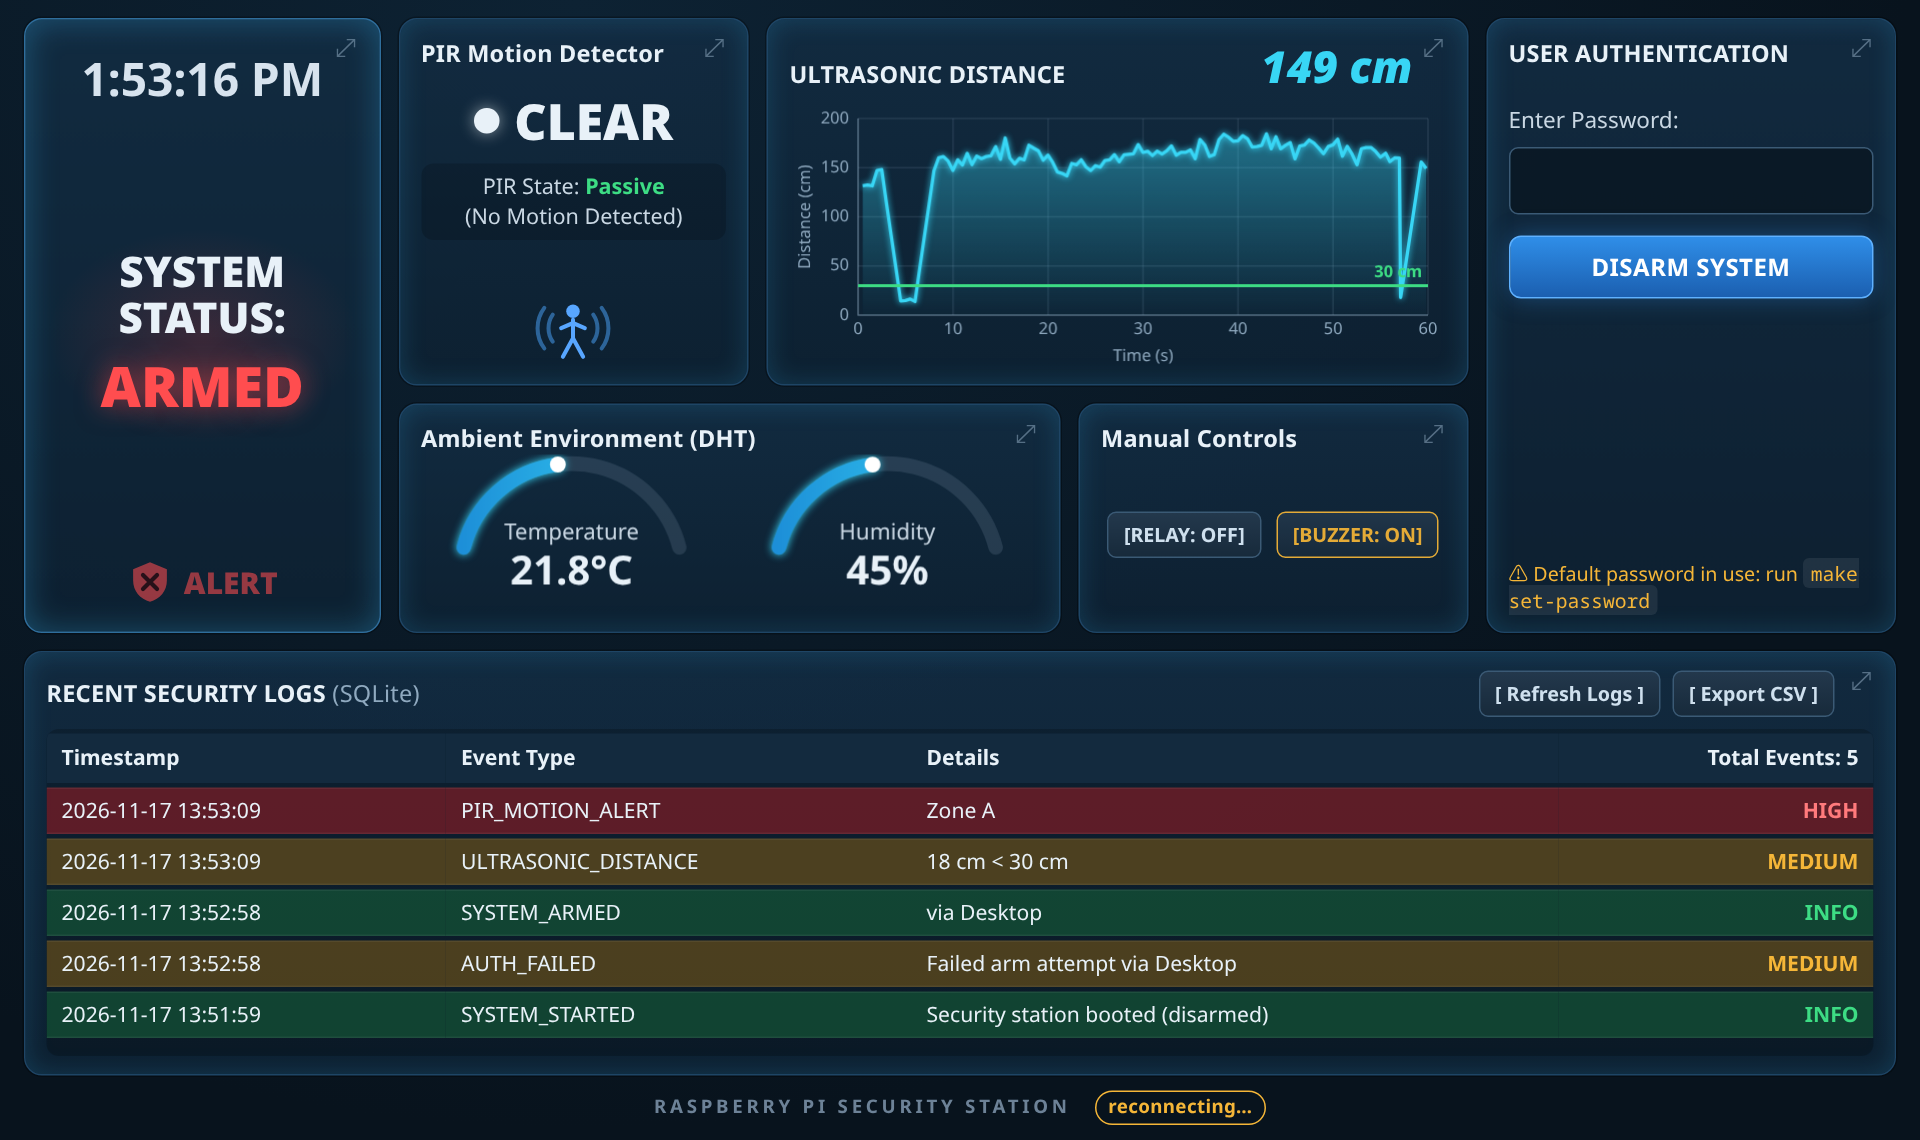
\includegraphics[width=\linewidth]{web_4_deconnexion.png}\end{subfigure}
\caption{\textbf{Déconnexion.} La station a été arrêtée. Sur le web, le badge en bas passe de
« live » (vert) à « reconnecting… » (orange), et la page se reconnecte seule au redémarrage. Les dernières
valeurs restent affichées. Ce signal est discret : un vrai bandeau d'erreur serait plus clair.}
\end{figure}

\begin{figure}[H]
\centering
\begin{subfigure}[t]{0.25\linewidth}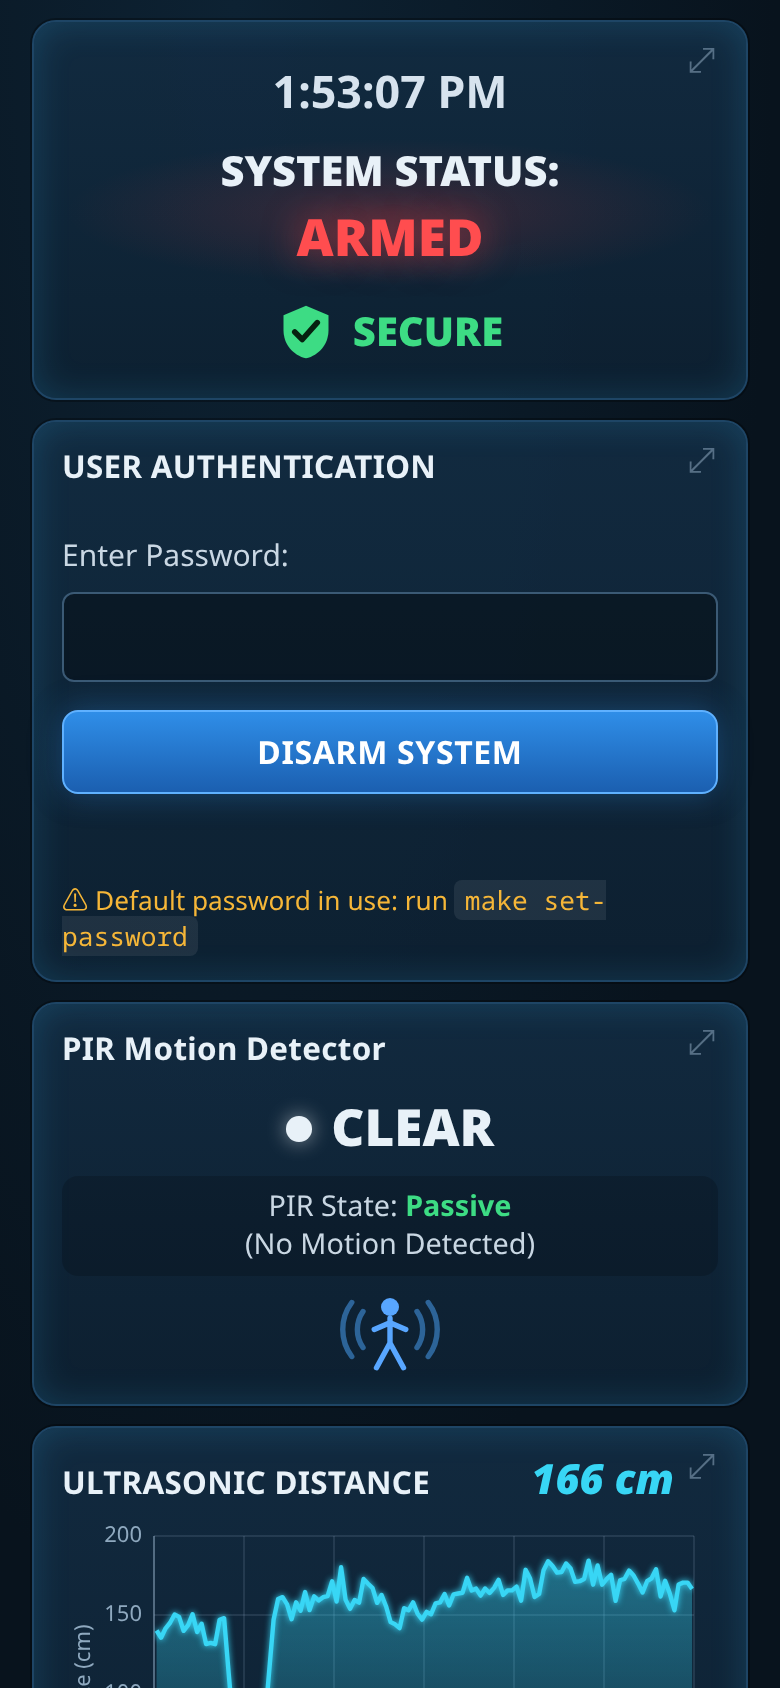
\includegraphics[width=\linewidth]{mobile_2_normal.png}\caption{Normal}\end{subfigure}\hspace{4mm}
\begin{subfigure}[t]{0.25\linewidth}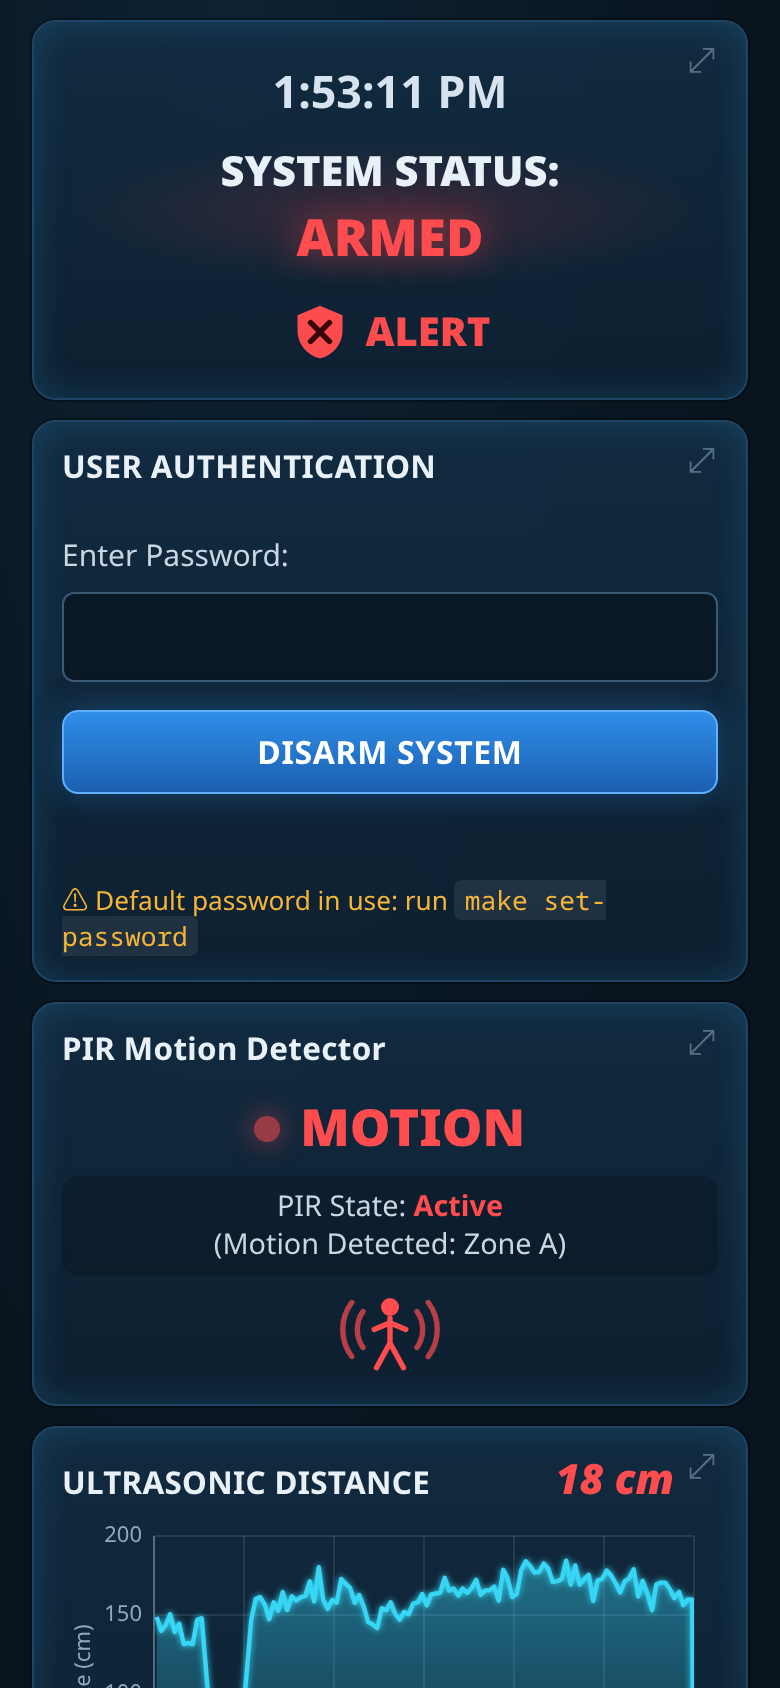
\includegraphics[width=\linewidth]{mobile_3_alarme.png}\caption{Alarme}\end{subfigure}\hspace{4mm}
\begin{subfigure}[t]{0.25\linewidth}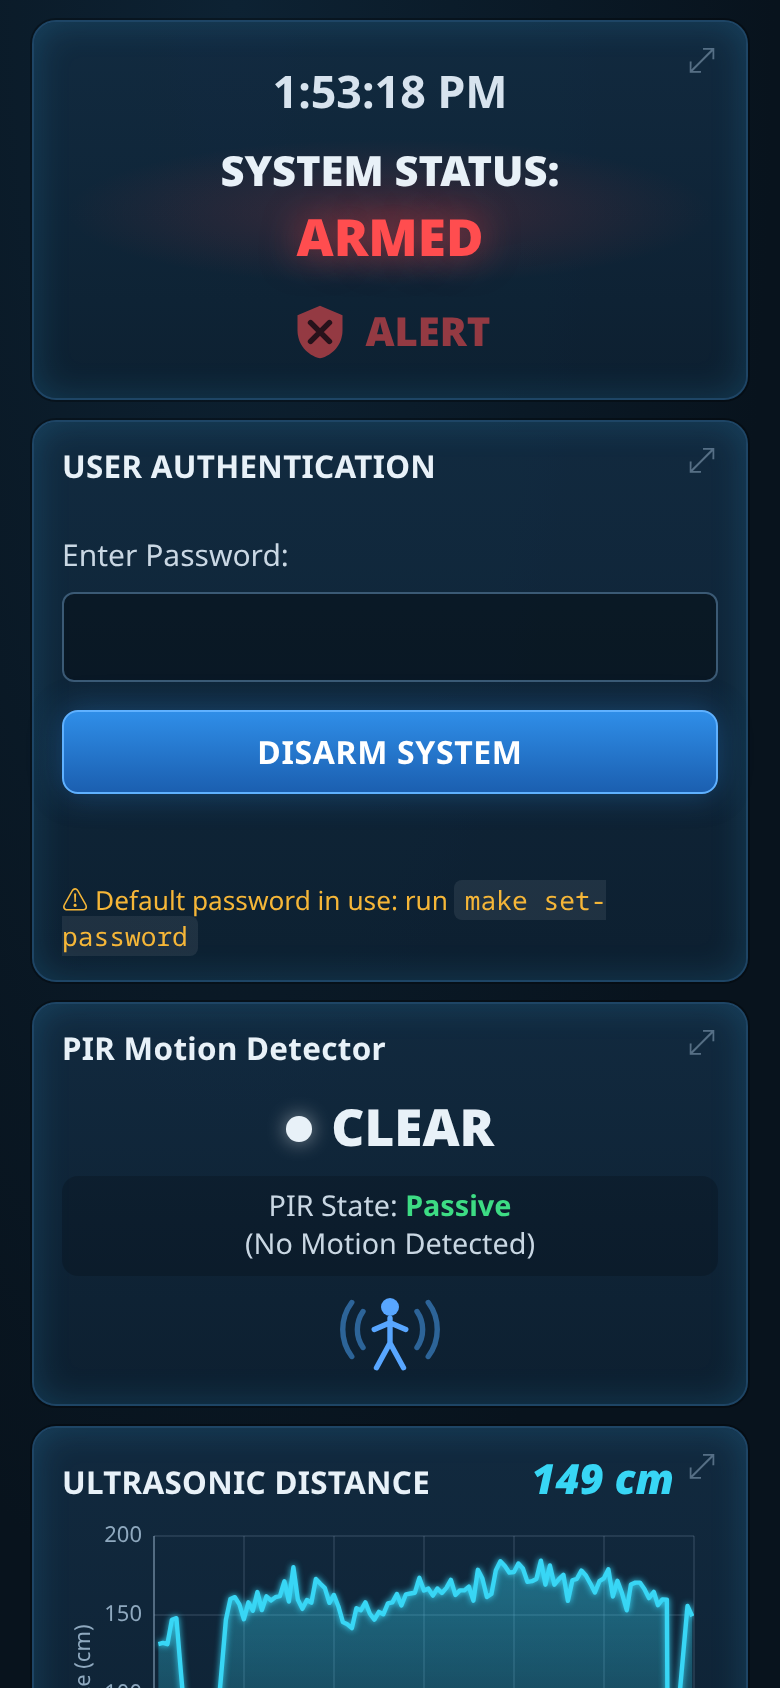
\includegraphics[width=\linewidth]{mobile_4_deconnexion.png}\caption{Déconnexion}\end{subfigure}
\caption{Interface web sur téléphone. Les tuiles se placent sur une seule colonne.}
\end{figure}

\paire{qt_5_vue_agrandie.png}{web_5_vue_agrandie.png}{\textbf{Tuiles agrandies.} Un clic sur une tuile ouvre une
grande vue avec plus de détails : statistiques de la distance (Qt), historique de 10 minutes de la température
et de l'humidité (web). « Back » ou Échap ramène au tableau de bord.}

% ======================================================================= conformité
\section{Conformité au cahier des charges}\label{sec:conformite}
\begin{table}[H]
\centering\small
\renewcommand{\arraystretch}{1.2}
\begin{tabularx}{\linewidth}{>{\raggedright}p{5.2cm} l >{\raggedright\arraybackslash}X}
\toprule
\textbf{Exigence} & \textbf{Fait ?} & \textbf{Commentaire} \\
\midrule
Au moins 2 capteurs & \ok & 3 capteurs simulés : ultrason, PIR, DHT22. \\
Au moins 1 actionneur & \ok & Relais et buzzer, visibles dans les interfaces et le journal. \\
Actionneurs émulés par des messages terminal & \non & L'état s'affiche dans les interfaces, pas dans le terminal. \\
Interface locale PySide6 & \ok & Tableau de bord fidèle à la maquette, tuiles agrandissables. \\
Interface conçue avec Qt Designer (\texttt{.ui}) & \non & Les écrans sont écrits directement en Python. \\
Mode kiosque (plein écran) & \ok & \texttt{make run-fullscreen} (F11 pour basculer). \\
Interface web réactive HTML5/CSS3 & \ok & S'adapte au PC, à la tablette et au téléphone. \\
Temps réel par WebSockets (FastAPI / Tornado) & \partiel & Temps réel assuré par SSE + HTTP, avec le serveur de la bibliothèque standard. \\
Commande des actionneurs à distance & \ok & Depuis le navigateur, avec mot de passe. \\
Synchronisation Qt $\leftrightarrow$ web & \ok & Une seule Station partagée ; mise à jour en moins d'une seconde. \\
Message clair en cas de déconnexion (web) & \partiel & Badge « reconnecting… » et reconnexion automatique, mais discret. \\
Base de données horodatée : événements d'alarme & \ok & Table \texttt{events}, limitée à 1000 lignes, export CSV. \\
Base de données : historique des relevés & \non & Les relevés restent en mémoire (60~s / 10~min). \\
Relevé continu & \ok & Mise à jour toutes les 0,5~s (ultrason) et 2~s (DHT). \\
Relevé unitaire sur demande & \non & Pas de bouton « lire maintenant ». \\
Min / Max / Moyenne sur les 10 derniers relevés en base & \partiel & Calculés sur les 60 dernières secondes, en mémoire. \\
Seuils d'alarme modifiables dans l'interface & \non & Seuil fixe (30~cm) dans \texttt{config.py}. \\
HAL (\texttt{SIMULATION\_MODE}, \texttt{ISensor}, \texttt{hal.py}) & \partiel & Simulation isolée dans un module, sans l'interface formelle. \\
Phase III : Pi réelle, câblage, vidéo physique & \hors & Seule la simulation a été réalisée. \\
\bottomrule
\end{tabularx}
\caption{Bilan par rapport au cahier des charges.}
\end{table}

\section{Conclusion et suite}
La station fonctionne entièrement en simulation : trois capteurs, deux actionneurs, une interface Qt et une
interface web synchronisées, un journal SQLite et un accès protégé par mot de passe.

Pour couvrir tout le cahier des charges, les prochaines étapes seraient :
\begin{enumerate}
  \item écrire la HAL du sujet (\texttt{ISensor}, \texttt{pseudo\_sensor.py}, \texttt{hal.py}) autour du simulateur actuel ;
  \item passer à FastAPI avec de vrais WebSockets ;
  \item enregistrer les relevés en base et calculer min, max et moyenne sur les 10 derniers ;
  \item ajouter les seuils modifiables, le relevé sur demande et un bandeau de déconnexion bien visible ;
  \item refaire les écrans dans Qt Designer (\texttt{.ui}) ;
  \item passer sur la Raspberry Pi avec les vrais capteurs (phase III).
\end{enumerate}

% ======================================================================= annexe
\appendix
\section{Annexe : lancer le projet}
\begin{lstlisting}[language=bash,numbers=none]
make setup            # crée l'environnement Python 3.13
make run              # fenêtre Qt + interface web (https://<ip>:8443)
make run-fullscreen   # mode kiosque sur l'écran de la Pi
make set-password     # change le mot de passe (par défaut : 1234)
make test             # lance les 40 tests
\end{lstlisting}
Au premier accès depuis un navigateur, il faut accepter une fois le certificat auto-signé.

\end{document}
